\begin{frame}
    \begin{center}
        \Huge{REST API}
    \end{center}
    \begin{figure}[h]
        \centering
        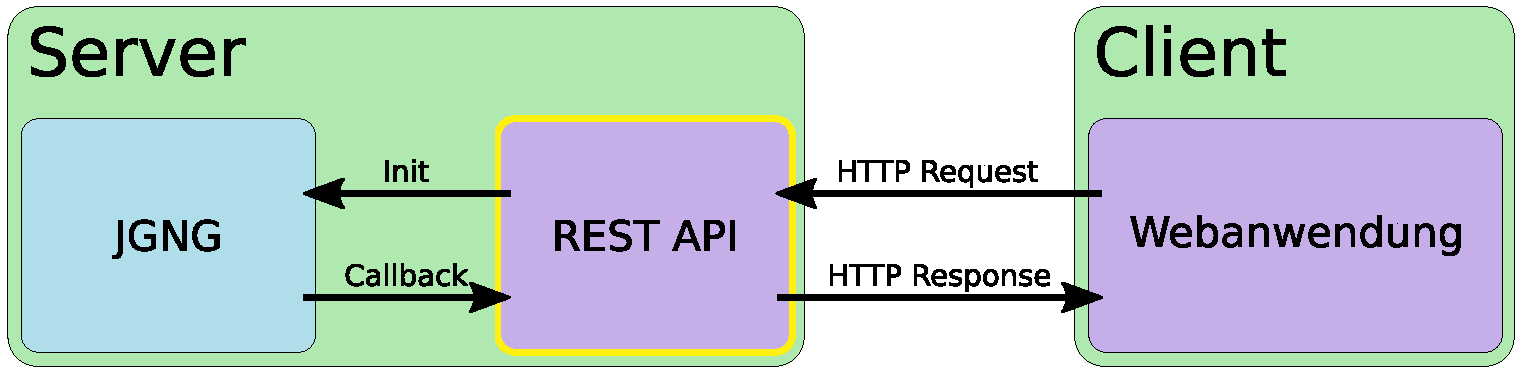
\includegraphics[width=\textwidth]{bilder/client-server_rest-active.pdf}
    \end{figure}
\end{frame}
\subsubsection*{Usecasediagramm API}
\begin{frame}
    \begin{figure}[h]
        \centering
        \includegraphics[width=0.6\textwidth]{../figures/apicontroller.pdf}
        \caption{Usecasediagramm API}
    \end{figure}
\end{frame}
%\subsection*{URL Struktur}
%\begin{frame}
%    \frametitle{URL Struktur}
%    \begin{center}
%        \begin{tabularx}{\textwidth}{ lll }
%            \textbf{HTTP-Methode} & \textbf{Pfad} & \textbf{Methode im Controller} \\
%            \hline
%            POST & \texttt{/training} & setTraining \\
%            POST & \texttt{/training/<id>} & setTrainingID \\
%            GET & \texttt{/training} & getTrainings \\
%            GET & \texttt{/training/<id>} & getTraining \\
%            PUT & \texttt{/training/<id>} & setSettings \\
%            DELETE & \texttt{/training/<id>} & deleteTraining \\
%            POST & \texttt{/train/<id>} & setTrain \\
%            GET & \texttt{/train/<id>} & getTrain
%        \end{tabularx}
%    \end{center}
%\end{frame}
\subsubsection*{Umsetzung}
\begin{frame}
    \frametitle{Aspekte der Implementierung}
    \begin{itemize}
        \item Initalisierung des JGNG
        \item Implementierung des Delegationsinterfaces(Callback)
        \item Datenstruktur für Neuronen und Kanten
        \item Verarbeiten der Nutzeranfragen und Bereitstellung der Daten
    \end{itemize}
\end{frame}
\begin{frame}
    \frametitle{JGNG Callback}
    \begin{figure}[h]
        \centering
        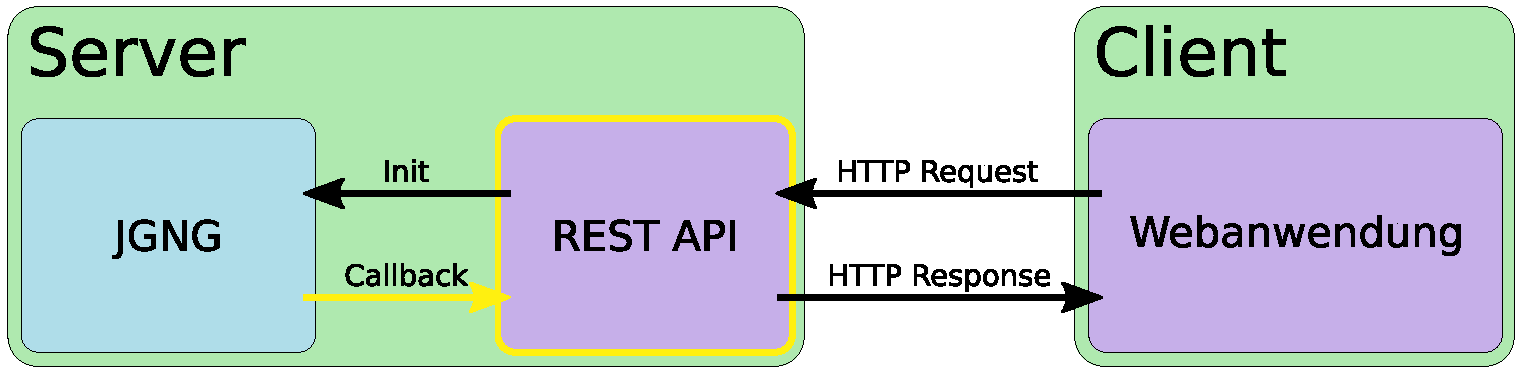
\includegraphics[width=\textwidth]{bilder/client-server_callback-active.pdf}
    \end{figure}
    \begin{itemize}
        \item Callback wird als Interface vom Algorithmus bereitgestellt und von der REST API impementiert
        \item Er empfängt alle Änderungen am neuronalem Netz
        \item \textbf{Problem:} NeuronenID sind nur Listindizes
        \newline $\rightarrow$ Mapping auf eindeutige IDs durch atomare Zählvariable
        \item Speicherung der Neuronen und Kanten
    \end{itemize}
\end{frame}
%\begin{frame}
%    \begin{figure}[h]
%        \centering
%        \includegraphics[width=\textwidth]{../figures/gngcallback.pdf}
%        \caption{Kommunikationsdiagramm GNGCallback}
%    \end{figure}
%\end{frame}
\begin{frame}
    \frametitle{Datenstruktur}
    \begin{itemize}
        \item Speicherung der Neuronen und Kanten als Objekte
        \newline $\rightarrow$ Verknüpfung mit zusätzlichen Attributen
        \item Zusammenfassung der Neuronen und Kanten in zwei verschiedenen Objekten
    \end{itemize}
    \begin{figure}[h]
        \centering
        \includegraphics[width=\textwidth]{../figures/datenstruktur.pdf}
        \caption{Klassendiagramm Datenstruktur}
    \end{figure}
\end{frame}
\begin{frame}
    \frametitle{Verwaltung der Anfragen}
    \begin{figure}[h]
        \centering
        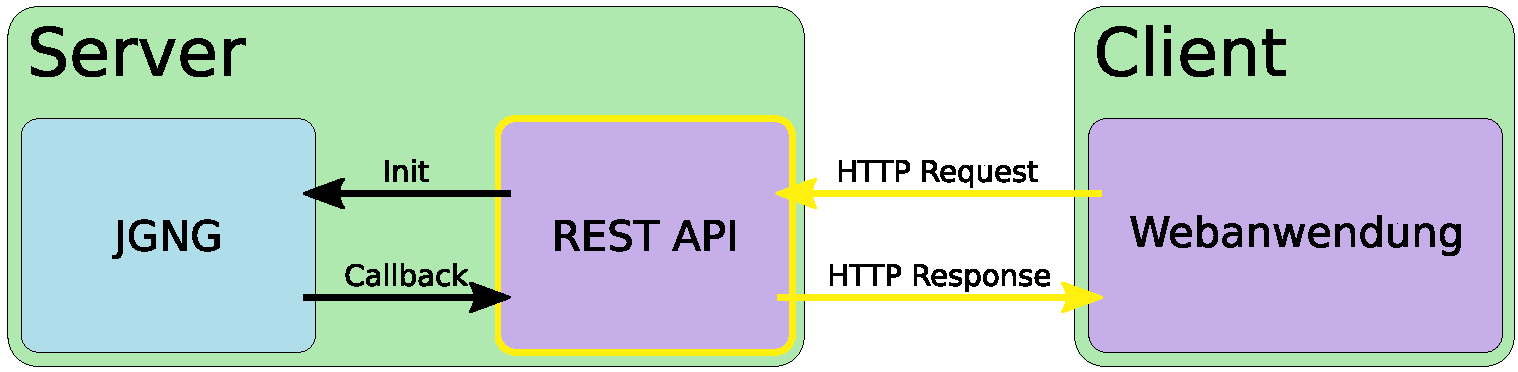
\includegraphics[width=\textwidth]{bilder/client-server_http-active.pdf}
    \end{figure}
    %\begin{center}
    %    \begin{footnotesize}
    %        \begin{tabularx}{\textwidth}{ lll }
    %            \textbf{HTTP-Methode} & \textbf{Pfad} & \textbf{Methode im Controller} \\
    %            \hline
    %            POST & \texttt{/training} & setTraining \\
    %            GET & \texttt{/training/<id>} & getTraining \\
    %            ... & &
    %        \end{tabularx}
    %    \end{footnotesize}
    %\end{center}
\end{frame}
\begin{frame}
    \frametitle{Einsatz des Spring Boot Framework}
    \begin{figure}[h]
        \centering
        \includegraphics[width=\textwidth]{../figures/springboot.pdf}
        %\caption{Spring Boot Framework}
    \end{figure}
\end{frame}
\begin{frame}
    \frametitle{REST Controller}
    Der REST Controller übernimmt folgende Aufgaben:
    \begin{itemize}
        \item Initialisierung des JGNG
        \begin{itemize}
            \item Kapselung des JGNG in einem Wrapper mit eindeutiger ID
            \newline $\rightarrow$ mehrere JGNG parallel verfügbar
            \item Übergabe eines Callback und Datenhaltung
        \end{itemize}
        \item Entgegennehmen der Einstellungen für das JGNG
        \item Zurückgeben des neuronalen Netzes
        \item Zurückgeben einer Trainingseinheit
    \end{itemize}
    Optional:
    \begin{itemize}
        \item Auflisten aller neuronalen Netze
        \item Löschen eines neuronalen Netzes
    \end{itemize}
\end{frame}
